%!TEX root = ../dokumentation.tex
\chapter{Theory}

\section{Kubernetes cluster solution}

One very common system for managing cluster systems as described in chapter 1.1 is \acl{K8s} - or short \acs{K8s}. Originally developed by Google and now maintained by the Cloud Native Computing Foundation, Kubernetes is an ``open-source platform for managing containerized workloads and services''.\textsuperscript{cmp.\cite{12}} For unterstanding what that means the concept of containers needs to be described first.

%https://kubernetes.io/docs/concepts/overview/what-is-kubernetes/

Containers are isolated, stand-alone packages of software, similar to processes. In those packages everything is included, which this piece of software needs, like runtime, libraries, settings and other system tools.  These containers have a completely different environment within themselves than outside. This environment includes for example network routes, dns settings and control group limits. This enables the possibility to share common resources and still be isolated from any other process as well as the host system. Thereby containers are always working the same, no matter on what system they run or in which environment.\textsuperscript{cmp.\cite{13}, \cite{14}}

%1 https://www.informatik-aktuell.de/entwicklung/methoden/kubernetes-architektur-und-einsatz-einfuehrung-mit-beispielen.html
%https://www.docker.com/what-container

Kubernetes is for an automating deployment, scaling and management of these containers within a cluster of nodes. Thereby a cluster consists of at least one master node and any number of worker nodes. Figure 2.1.1 shows the different services owned by master and worker nodes.

\begin{figure}[h]
\centering
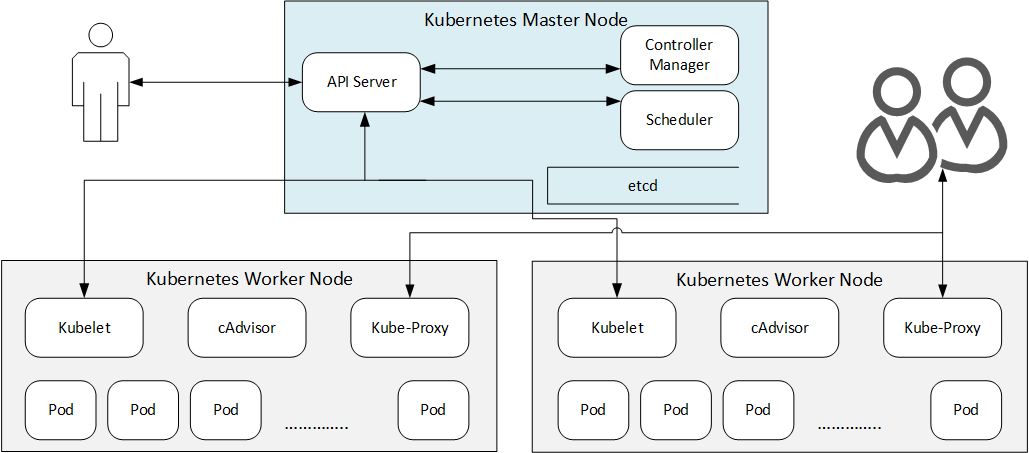
\includegraphics[width=\textwidth/5*3]{images/kubernetes_service_allocation.png}

\textsuperscript{Figure 2.1.1 Kubernetes allocation of services}\\
\textsuperscript{Based on retrieved information from \cite{13}}
\end{figure}

First there are several pods on each worker node. Pods are the smallest unit in Kubernetes. They contain one or more containers, which are deployed together on the same host. Thereby they can work together to perform a set of tasks.\textsuperscript{cmp.\cite{15}}%more?
%https://coreos.com/kubernetes/docs/latest/pods.html

On the master node there are an \acs{API} (\acl{API}) Server, a Controller Manager, a Scheduler and a key-value store called etcd.\textsuperscript{cmp.\cite{13}, \cite{16}}

The API Server is for clients to run their requests against. That means the API Server is responsible for the communication between Master and Worker nodes and for updating corresponding objects in the etcd. Also the authentication and authorization is task of the API Server. The protocol for the communication is written in \acs{REST} (\acl{REST}). For reacting on changes of clients there is also a watch mechanism implemented, which triggers an action after some specific changes, like the scheduler creating a new pod. This workflow is showed in figure 2.1.2.\textsuperscript{cmp.\cite{13}, \cite{16}}

\begin{figure}[h]
\centering
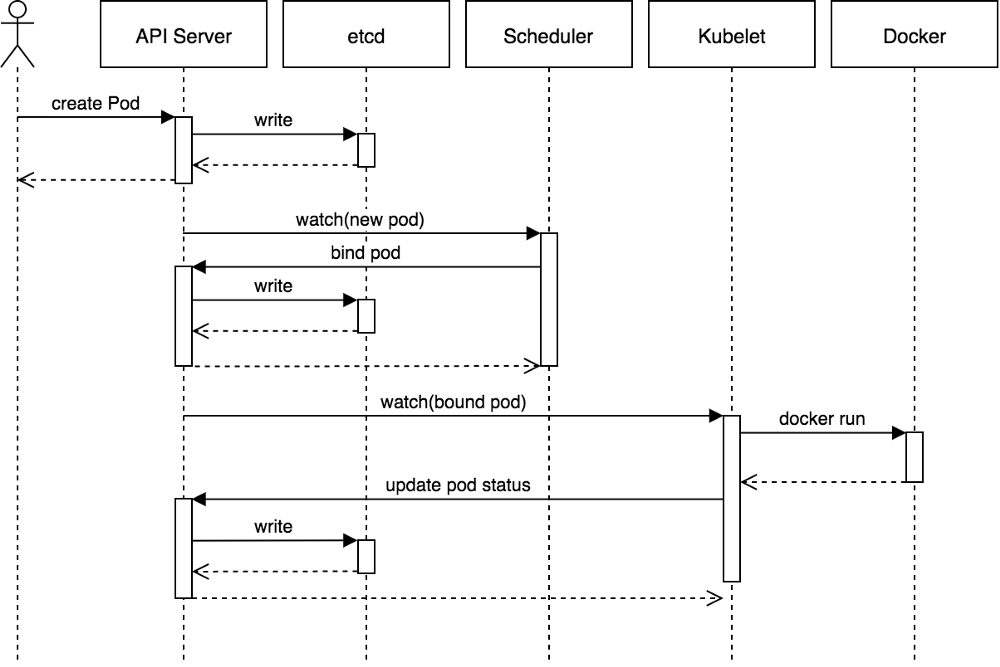
\includegraphics[width=\textwidth]{images/kubernetes_watcher_sequence.png}

\textsuperscript{Figure 2.1.2 Kubernetes API Server watcher sequence diagram}\\
\textsuperscript{Based on retrieved information from \cite{16}}
\end{figure}

There you can see the user creating a pod through a belonging request to the API Server. The API Server writes this change to the etcd. Afterwards the API Server recognizes a new pod in the etcd and invokes the Scheduler to create this new pod. What is the exact task of the scheduler is described later. After successfully creating and binding the new pod, the API Server writes this change to the etcd. Because of this change within the etcd the API Server invokes the kubelet, which is also described later in this chapter, of the corresponding node. This kubelet starts docker to create the containers of the pod. Kubelet responses with the new status of the pod, which is then written to the etcd by the API Server. After that the creation of the new pod is successfully finished.\textsuperscript{cmp.\cite{13}, \cite{16}}

The Controller Manager is a daemon, which embeds all of the Kubernetes controller. Examples for them are the Replication Controller or the Endpoint Controller. Those controllers are watching the state of the cluster through the API Server. Whenever a specific action happens, it performs the necessary actions to hold the current state or to move the cluster towards the desired state. For providing an example: If the Replication Controller recognizes, that one replication of a pod has been destroyed for some reason, it will take care of triggering the creation of a new replication.\textsuperscript{cmp.\cite{13}, \cite{16}}

The scheduler manages the binding of pods to nodes. Therefore it watches for new deployments as well as for old ones to create new pods if a new deployment is created or recreating a pod whenever a pod gets destroyed. The scheduler organizes the allocation of the pods within the cluster on the basis of available ressources of the pods. That means, that it always create pods, where the most resources are available, or reorganize the allocation if there is a change in the resource allocation of the cluster.\textsuperscript{cmp.\cite{13}, \cite{16}}%??

Figure 2.1.3 shows the way the Scheduler works, when new nodes are connected. As long as there are only two nodes and four pods need to be deployed, it allocates those four pods to the two nodes . As soon as there are more nodes connected, the scheduler recognizes free resources and reallocate the pods to these new nodes.

\begin{figure}[h]
\centering
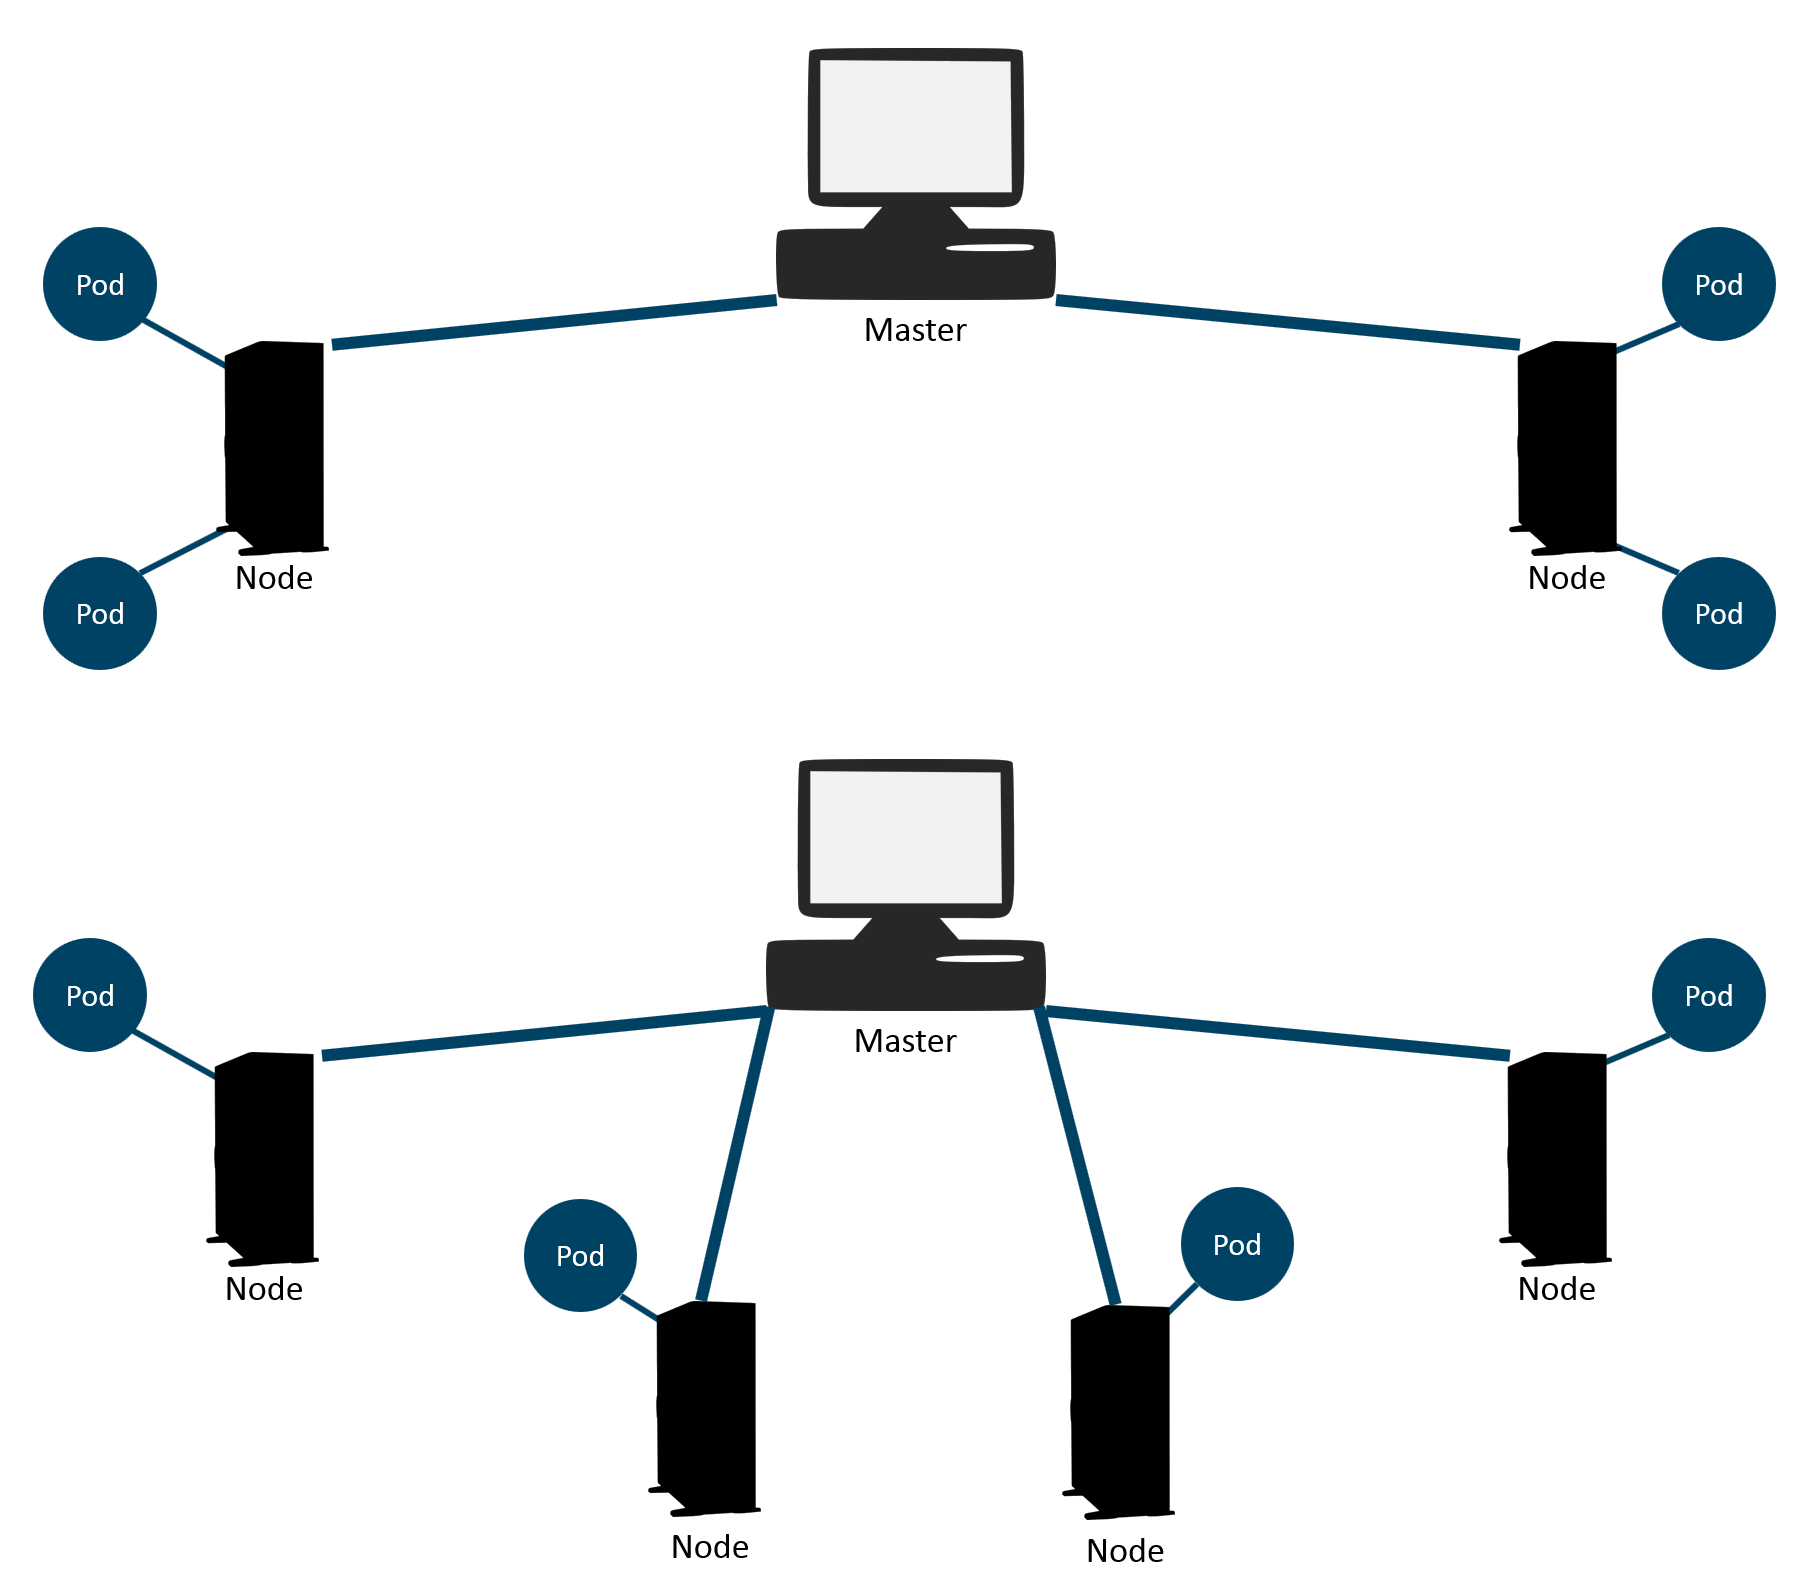
\includegraphics[width=\textwidth/5*3]{images/kubernetes_scheduler.png}

\textsuperscript{Figure 2.1.3 Kubernetes API Server watcher sequence diagram} \\
\textsuperscript{Based on retrieved information from \cite{17}}
\end{figure}
%https://www.informatik-aktuell.de/fileadmin/_processed_/b/6/csm_K8s_abb1_fricke_b5ce6bd912.png

The etcd is a key-value store, which stores the configuration data and the condition of the Kubernetes cluster. The etcd also contains a watch feature, which listens to changes to keys and triggers the API server to perform all necessary actions to move the current state of the cluster towards the desired state.\textsuperscript{cmp.\cite{13}, \cite{16}}

The worker node consists of a Kubelet, a cAdvisor, a Kube-Proxy and - as mentioned before - several Pods. 

The kubelet needs to be used if a new pod should be deployed. Then it gets the action to create all needed containers. For that it uses Docker to create them. Afterwards it combines some containers into one pod. Conainers in one pod are always started and stopped together. This pod will then be deployed on the node, on which the kubelet is located.\textsuperscript{cmp.\cite{13}, \cite{16}}

The cAdvisor measures the usage of CPU-resources as well as demanded memory on the node, on which it is located, and notifies the master about it. Based on those measurements the scheduler allocates the pods within the cluster to ensure the best possible allocation of resources.\textsuperscript{cmp.\cite{13}, \cite{16}}

The kube-proxy is a daemon, that runs as a simple network proxy to provide the possibility of communicating to that node within the cluster. Additionally it runs a load balancer for the services on that node.\textsuperscript{cmp.\cite{13}, \cite{16}}

Through this architecture Kubernetes enables different possibilities to deploy pods within the cluster. The simplest one is to deploy a specific pod directly through the 
\begin{lstlisting}[caption={Create Kubernetes pod},captionpos=b]
kubectl create -f `image\_path'
\end{lstlisting}
command. This deploys the pod described in the file, but it doesn't ensure the failure safety. That means if the pod gets destroyed for some reason, no matter if it has been destroyed by accident or intended, it won't be recreated and deployed again automatically. 

%1
%2 https://medium.com/jorgeacetozi/kubernetes-master-components-etcd-api-server-controller-manager-and-scheduler-3a0179fc8186

Another possibility is to create a deployment. Therefore the image has to be embedded within a replicaset and this replicaset within a deployment. If this deployment is created, it will automatically create every pod of the replicaset. If one pod gets terminated, no matter if manually or because of an error, it will be directly recreated and deployed.\textsuperscript{cmp.\cite{13}, \cite{18}}

This procedure also enables the possibility to execute dynamical rolling updates. If you execute the command
\begin{lstlisting}[caption={Create Kubernetes deployment},captionpos=b]
kubectl set image deployment/name-deployment name=name:1.1.1
\end{lstlisting}
Kubernetes will start a Rolling Update. This causes the creation of a new replicaset, which uses pods of the new version. While the new replicaset will be scaled up, the old one will be scaled down step by step. This enables the maintenance of a deployment even while an update is enrolled, so that the users can still use the services while those are updating. That means, that there is never a need of a system to shut down because of an update, which needs to be enrolled, and the system guarantees its high availability.\textsuperscript{cmp.\cite{13}, \cite{18}}

A third possibility to deploy pods are services. Services are used to enable the usage of pods from outside the cluster. Therefore it gets the pod from the targetPort of the belonging node and creates a random port on this node. This port serves as endpoint for the LoadBalancer. Through this, everybody can now communicate with this pod.\textsuperscript{cmp.\cite{13}, \cite{18}}

This is how Kubernetes ensures High Availability as well as Load Balancing at the same time. Through the possibility of replicate every pod several times it is ensured that whenever one pod fails for some reason, another is already prepared to help out and take over the job. Even the master can and should be replicated to ensure a functional system, even if one master has been destroyed. For production environment it's recommended to have 3, 5 or 7 master nodes running at the same time. For facilitating the High Availability almost every unit of a Kubernetes cluster is stateless and could be run redundant in several instances. Only the etcd key value store is stateful. For solving that problem in case of failure of the node, which owns the etcd, there is a leader election between all master node replicas to determine the new leading etcd.\textsuperscript{cmp.\cite{13}, \cite{18}}

%1
%2
%https://deis.com/blog/2016/kubernetes-overview-pt-1/

All in all Kubernetes combines all the benefits of cluster applications in one software. High availability as well as load balancing is guaranteed and it also ensures a high scalability, rolling updates and auto-scaling. Compared to other cluster systems, like Docker swarm, it has the biggest community and it can support clusters of up to 5000 nodes, which enables using Kubernetes even for very big clusters. For example the whole Google Cloud System runs on a Kubernetes cluster. Performing tests of Kubernetes shows, that in 99\% the API responses in less than one second and also their pods start in less than five seconds in 99\% when starting containers with pre pulled images. This all makes Kubernetes maybe one of the most flexible and fastest cluster systems. In exchange for that flexibility it is more difficult to set it up, because you have to do it all on your own. But only that way it can be ensured, that it runs fast and flexible in the same time, which is the reason for Kubernetes being so popular.\textsuperscript{cmp.\cite{19}, \cite{20}}

%https://platform9.com/blog/kubernetes-docker-swarm-compared
%https://www.redhat.com/de/topics/containers/what-is-kubernetes ???

%Storage?

\section{Spark}

Apache Spark is an open source framework for big data analytics and large-scale data processing. It supports \acs{SQL} (\acl{SQL}), streaming data, machine learning and graph processing. It is working as a framework used in clusters. Therefore it offers native support for Hadoop YARN, Apache Mesos and since version 2.2.0 also Kubernetes.\textsuperscript{cmp.\cite{21}}

%https://apache-spark-on-k8s.github.io/userdocs/running-on-kubernetes.html

Spark is known as a very fast data processing system, which is caused by its in-memory processing capability. This is the big advantage of Spark in comparison to other Big Data Analysis tools like Apache Hadoop. Hadoop uses distributed storage mechanism instead of in-memory processing. This was very successful at the beginning of the Bid Data warehouse era, but with the possibility to run in-memory calculations Spark has a big advantage nowadays. By official information of Apache Spark, Spark is capable of 100 times faster workload runs than Hadoop.\textsuperscript{cmp.\cite{22}}

%https://spark.apache.org/

Another advantage of Spark is its easy cloud-based implementation, which enables companies to run their analysis of their data directly on the Cloud instead of using local devices for it. Through this the companies don't have to have two copies of their data, on which they can run their calculations on, but they can do everything directly on the Cloud.\textsuperscript{cmp.\cite{23}}

%https://tdwi.org/articles/2018/06/22/ta-all-apache-spark-and-big-data-whats-ahead.aspx
%NACHLESEN!!

For ensuring all of these features work - no matter on what cluster system - Spark applications are split in independent sets of processes on such a cluster. Figure 2.2.1 shows how this works and how the processes are coordinated.

\begin{figure}[h]
\centering
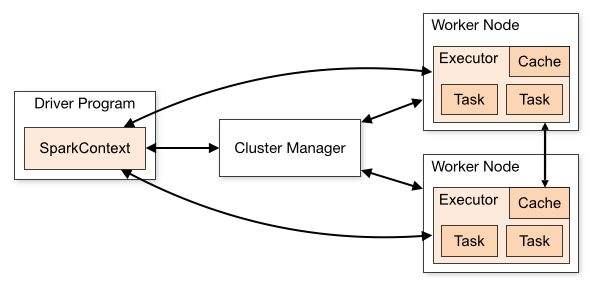
\includegraphics[width=\textwidth/4*3]{images/spark_cluster_architecture.png}

\textsuperscript{Figure 2.2.1 Spark cluster architecture\cite{24}}
\end{figure}
%https://spark.apache.org/docs/latest/img/cluster-overview.png

First there is the SparkContext in the main program, also called driver program. This context coordinates all the processes. Therefore it connects to the cluster manager of the cluster system which is used (Mesos, Yarn or Kubernetes). As described in chapter 2.1. their task is to allocate processes based on free resources of the nodes within the cluster. Spark then spawns executors on the nodes of the cluster. Executors are processes on which the applications are running. After that it also sends the application code to the executors and give them tasks to run. While they are running, the executors can also store data for the application.\textsuperscript{cmp.\cite{25}}

This architecture with several independent executors has the big advantage, that isolated applications can run in multiple threads at the same time. Combined with the in-memory-processing this guarantees enormous speed and a great overall-performance.

Spark usually persists out of six different components - the Spark Core, Spark \acs{RDD}, Spark SQL, Spark Streaming, MLlib Machine Learning and GraphX.

Spark Core is the base of the overall project and offers distributed task dispatching, scheduling and basic \acs{I/O} (\acl{I/O}) functionalities. Every other component is based on this core.\textsuperscript{cmp.\cite{26}, \cite{28}}

The first of them is Spark RDD - \acl{RDD}. RDD represents a collection of objects, which are spread across the cluster. This enables the possibility of fast and scalable data algorithms, because operations on these objects can be distributed within the cluster.\textsuperscript{cmp.\cite{26}, \cite{28}}

Spark SQL provides a SQL compliant interface for querying data - so there is default, but limited SQL support in Spark. It also enables processing of structured data inside Spark. Additionally Spark SQL provides an interface for reading from and writing to other dataformats like \acs{JSON} (\acl{JSON}) or Apache Parquet and other datastores like \acs{HDFS} (\acl{HDFS}) out of the box. For other stores like Apache Cassandra or MongoDB there are Spark Packages available in its ecosystem.\textsuperscript{cmp.\cite{26}, \cite{28}}

Spark Streaming helps Spark in environments for real-time processing. Therefore it breaks the stream down into a continuous series of microbatches. Microbatches are nothing else than a very small group of data elements, which will be processed at once after being collected.\textsuperscript{cmp.\cite{26}, \cite{28}}These microbatches can then be manipulated using the Spark API. Through this streaming, operations can share mostly the same code and run on the same framework.\textsuperscript{cmp.\cite{27}}
%https://streaml.io/resources/tutorials/concepts/understanding-batch-microbatch-streaming/

The MLlib is a library for machine learning for Spark. It includes a framework for machine learning algorithms and pipelines. It comes with a variety of tasks like featurization, transformations, model training and optimization.\textsuperscript{cmp.\cite{26}, \cite{28}}

GraphX provides a library for large-scale graph analytics. If offers an efficient abstraction for representing graph-oriented data and comes with various graph transformations, common graph algorithms and a collection of graph builders.\textsuperscript{cmp.\cite{26}, \cite{28}}

This all makes Spark to a very extensive tool for big data analysis. But there are still some features missing, like traditional ACID transactions or an enterprise-quality SQL service. One way to solve that problem is described in chapter 2.3.


%https://spark.apache.org/docs/latest/cluster-overview.html
%https://www.infoworld.com/article/3236869/analytics/what-is-apache-spark-the-big-data-analytics-platform-explained.html
%https://link.springer.com/content/pdf/10.1007%2Fs41060-016-0027-9.pdf

\section{Wildfire}

As already introduced in chapter 1.1 there are different kinds of data processing systems - OLAP and OLTP. To combine those two systems HTAP has been developed and Wildfire is an HTAP system developed by IBM in Almaden.

Wildfire brings OLTP features to the OLAP system Spark. Thereby Wildfire uses Spark to perform analytics, using and extending Spark APIs for SQL queries and automatically replicating data for high availability, scale-out performance and elasticity. Wildfire expands these functionalities with features like ACID transactions with snapshot isolation, making the last committed data immediately available to analytics queries; indexing any column for fast point queries and enterprise-quality SQL.\textsuperscript{cmp.\cite{29}}
%quiote?
Wildfire consists of Spark itself at the one hand and the Wildfire engine at the other hand. The main entry point for every application targeted by Wildfire is Spark. Spark also provides all its common features for big data analytics. The Wildfire engine extends these functionalities by enabling analytics on newly ingested data as well and accelerating the processing of application requests. Wildfire extends Spark with a new OLTP API for OLTP workarounds. Each request spawns Spark executors across the used cluster. The used node depends upon the type of that request.\textsuperscript{cmp.\cite{29}}

\begin{figure}[h]
\centering
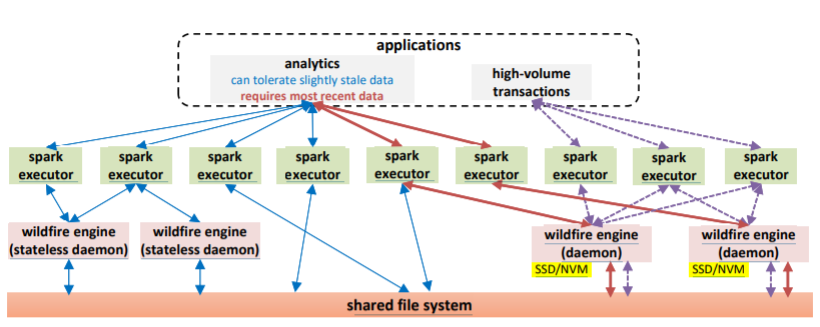
\includegraphics[width=\textwidth]{images/wildfire_architecture.png}

\textsuperscript{Figure 2.3.1 Wildfire architecture}\textsuperscript{cmp.\cite{29}}
\end{figure}

In figure 2.3.1 the architecture of the Wildfire HTAP system is shown. There can be seen several spawned executors of Spark. Most of them are for executing analytical requests only. Only some, beefier nodes with faster local persistent storage like SSDs and more cores for increased parallelism handle both - transactional and analytical queries on the recent data from those transactions. In this figure transaction requests are indicated by dashed arrows, while every other executor for analytics only are indicated by solid arrows.\textsuperscript{cmp.\cite{29}}

Additionally the figures shows several Wildfire engine instance daemons. Each of them is connected to at least one Spark executor. The stateless daemons are only connected to analytical-only executors, while the stateful daemons are connected to one or more executors for high volume transactions and to analytics executors for the most recent data. Those are indicated by red arrows. For that reason the stateless daemons are obviously for analytics queries on the much more voluminous older data while the stateful daemons handle transactions as well as analytics request against the latest data.\textsuperscript{cmp.\cite{29}}

For persisting and reusing those data for later queries, there is a shared file system, on which every daemon, no matter if stateful or stateless, has access to.%more?

%https://researcher.watson.ibm.com/researcher/files/us-ytian/wildfire-cidr17.pdf

In Wildfire the data are stored as tables defined with a primary key, a sharding key and optionally a partition key. The sharding key is a subset of the primary key and it is primary used for load balancing of transaction processing. A shard of a table is replicated into multiple nodes, but only one replica serves as the shard leader, the rest are slaves. A table shard is the basic unit of a lot of processes like grooming, post-grooming and indexing. The partition key is for organizing data for analytical queries to speed up time-based analytics queries.\textsuperscript{cmp.\cite{29}, \cite{30}}

For keeping track of the life of each record Wildfire adds three hidden columns to every table - \acs{beginTS} (\acl{beginTS}; time when record is first ingested), \acs{endTS} (end timestamp; time when the record is replaced by a new record with the same primary key) and \acs{prevRID} (previous record ID; record ID of the new record, who replaces this record). \textsuperscript{cmp.\cite{29}, \cite{30}}

For supporting both data processing systems (OLTP and OLAP) efficiently, Wildfire divides data into multiple zones. That way transactions can first apend their updates to the OLTP friendly zone, which are then migrated to the OLAP friendly zone step by step. Figure 2.3.2 shows the lifecycle of those stages.

\begin{figure}[h]
\centering
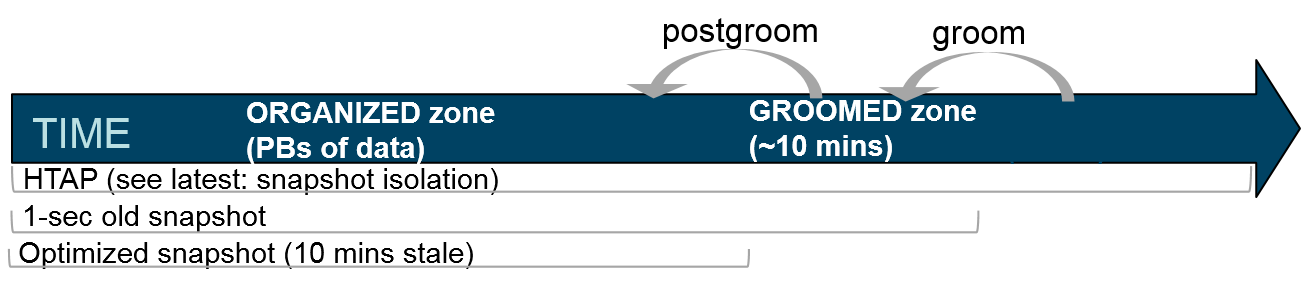
\includegraphics[width=\textwidth]{images/wildfire_lifecycle.png}

\textsuperscript{Figure 2.3.2 Wildfire lifecycle \cite{9}}
\end{figure}

First there is the life zone, where the transaction first appends uncommited changes in a transaction local side-log. Thereby it sets the beginTS for each record and appends its side-log to the committed transaction log. This log is kept in memory for fast access and also persisted on the local SSDs using the Parquet columnar-format. This zone always has the latest ingested data.\textsuperscript{cmp.\cite{30}}

After that, WIldfire periodically invokes a groom operation (e.g. every second) to migrate data from the live zone to the groomed zone. This operation merges transaction logs from shard replicas, resolves conflicts and creates a Parquet columnar-format data file, called a groomed black, in the shared storage. Each groomed block can be identified by a monotonic increasing ID called groomed block ID. The groomer also builds indexes over the groomed data and set the higher order part of the beginTS. The lower part will remain the transaction time in the shard replica.\textsuperscript{cmp.\cite{30}}

Last Wildfire periodically performs the post-grooming operation (e.g. every 10 minutes) to set the endTS and prevRID and reorganize the data to a more analytics-friendly way ba a partition key. This zone is called post-groomed or organized zone. This operation first utilizes the post-groomed portion of the indexes to collect the RIDs of the already post-groomed records, that will be replaced. Then it scans the newly groomed blocks to set prevRID fields and reorganizes the data into post-groomed blocks on the shared storage according to the OLAP friendly partition key. It usually generates much larger blocks than the groomer, because it is carried out less frequently. This results in better access performance on shared storage. Last the post-groomer also notifies the indexer process to build indexes on the newly post-groomed blocks.\textsuperscript{cmp.\cite{30}}

All in all this means that there is one live zone, which always have the newest ingested data, a groomed zone, which owns an one second old snapshot of the data, and an organized zone, which owns a ten minutes old snapshot, but which is optimized for analytic processes. Through this stations the data will be in an OLTP-friendly as well as in an OLAP-friendly form, so that it enables analytics and transactional processes at the same time. 

%index paper

